\documentclass[conference]{IEEEtran}
\IEEEoverridecommandlockouts
% The preceding line is only needed to identify funding in the first footnote. If that is unneeded, please comment it out.
\usepackage{cite}
\usepackage{amsmath,amssymb,amsfonts}
\usepackage{algorithmic}
\usepackage{graphicx}
\usepackage{textcomp}
\usepackage[utf8]{vietnam}
\usepackage[table]{xcolor}
\usepackage{multirow}
\usepackage{multicol}
\usepackage{float}
\usepackage{xurl} 

\def\BibTeX{{\rm B\kern-.05em{\sc i\kern-.025em b}\kern-.08em
    T\kern-.1667em\lower.7ex\hbox{E}\kern-.125emX}}
\begin{document}

\title{Dự báo giá của tiền điện tử bằng phương pháp chuỗi thời gian}
\maketitle

\begin{abstract}
Nghiên cứu này sử dụng một loạt các mô hình dự báo để phân tích và dự đoán tỷ giá trao đổi của Binance Coin (BNB), Bitcoin (BTC), và Ethereum (ETH) so với USD từ năm 2019 đến 2024. Bằng cách sử dụng các mô hình như TimesNet, Random Forest, CNN-LSTM, Bagging Model, và VAR để dự báo các biến động, cùng với hồi quy tuyến tính, nghiên cứu của chúng tôi nhằm cung cấp những thông tin quý báu cho các nhà đầu tư, các nhà phân tích tài chính, và những nhà quyết định chính sách trong việc điều hướng thị trường tiền điện tử dao động mạnh mẽ.
\end{abstract}

\begin{IEEEkeywords}
Chuỗi thời gian, phương pháp thống kê, tỷ giá trao đổi tiền điện tử, học máy, học sâu
\end{IEEEkeywords}

\section{Giới thiệu}
Trong thời đại hiện nay, thị trường tiền điện tử đã trở thành một phần không thể thiếu của hệ thống tài chính toàn cầu, và việc theo dõi và dự báo tỷ giá trao đổi của tiền điện tử so với USD là vô cùng quan trọng. Trong phạm vi này, nhóm tập trung vào ba loại tiền điện tử phổ biến nhất: Binance Coin (BNB), Bitcoin (BTC), và Ethereum (ETH).

Nghiên cứu này sẽ sử dụng một loạt các mô hình dự báo để hiểu và dự đoán các biến động trong tỷ giá trao đổi của các loại tiền điện tử này so với USD. Cụ thể, nhóm sẽ sử dụng các mô hình hồi quy tuyến tính để phân tích các xu hướng dài hạn, và sau đó sử dụng các mạng nơ-ron như TimesNet và CNN-LSTM để khám phá mối quan hệ phức tạp giữa các yếu tố và dự báo các biến động ngắn hạn.

Ngoài ra, nhóm cũng sẽ áp dụng các mô hình học máy như Random Forest, XGBoost, và VAR (Vector Autoregression) để đảm bảo tính linh hoạt và độ chính xác trong việc dự báo. Sự kết hợp của những mô hình này sẽ cung cấp một cái nhìn toàn diện về các xu hướng và biến động trong tỷ giá trao đổi của tiền điện tử so với USD, giúp các nhà đầu tư và chuyên gia tài chính đưa ra quyết định đầu tư thông minh và hiệu quả.

\section{Nghiên cứu liên quan}

Có một số nghiên cứu đã được thực hiện về chủ đề này:\par
Yecheng Yao và cộng sự \cite{b1} đã đề xuất một cách tiếp cận học sâu để dự đoán giá của tiền điện tử. Bài báo này tập trung vào việc sử dụng Long Short-Term Memory (LSTM) và Recurrent Neural Network (RNN) để phân tích dự báo giá của tiền điện tử. Các yếu tố được xem xét bao gồm vốn hóa thị trường, khối lượng giao dịch, nguồn cung lưu thông và nguồn cung tối đa. Tác giả cũng đề cập đến một số yếu tố như môi trường chính trị và quy định của con người.\par
Muhammad Ali Nasir và cộng sự \cite{b2} đã đề xuất một mô hình trong đó lợi suất và khối lượng của tiền điện tử được dự đoán bằng cách sử dụng các công cụ tìm kiếm. Một tập dữ liệu hàng tuần từ năm 2013 đến 2017 được sử dụng và thu thập cấu trúc phụ thuộc bằng cách sử dụng các phương pháp kinh nghiệm như VAR framework, một phương pháp copulas vv.\par
Aggarwal A. và cộng sự \cite{b3} đã thảo luận về các thông số khác nhau ảnh hưởng đến dự đoán giá Bitcoin dựa trên Root Mean Square Error (RMSE) sử dụng các mô hình học sâu như Convolutional Neural Network (CNN), Long ShortTerm Memory (LSTM) và Gated Recurrent Unit (GRU).\par
Alessandretti, L., ElBahrawy, A., Aiello, L.M. và Baronchelli, A. \cite{b4} đã kiểm tra hiệu suất của ba mô hình trong việc dự đoán giá tiền điện tử hàng ngày cho 1681 loại tiền điện tử. Hai trong số các mô hình dựa trên cây quyết định tăng cường độ dốc và một dựa trên Long ShortTerm memory. Trong tất cả các trường hợp, các danh mục đầu tư được xây dựng dựa trên các dự đoán và hiệu suất được so sánh dựa trên lợi nhuận từ đầu tư.\par
Mittal R. và cộng sự \cite{b5} đã dự đoán giá của tiền điện tử dựa trên giá mở, giá thấp và giá cao của chúng. Một số thuật toán Machine Leaning được sử dụng để dự đoán các thay đổi giá hàng ngày của tiền điện tử. Bộ dữ liệu được sử dụng trong bài báo này là tương đối nhỏ. Hồi quy tuyến tính đa biến đã được sử dụng để dự đoán giá cao nhất và thấp nhất của tiền điện tử.\par
Suhwanji và cộng sự \cite{b6} đã phát triển và so sánh các mô hình dự đoán giá Bitcoin dựa trên thông tin blockchain Bitcoin. Cụ thể, họ đã kiểm tra các mô hình học sâu tiên tiến như mạng nơ-ron sâu (DNN), mô hình long short-term memory (LSTM), mạng nơ-ron tích chập (CNN), mạng nơ-ron còn sót (ResNet) và các sự kết hợp của chúng. Đối với các vấn đề hồi quy, LSTM đạt hiệu suất tốt hơn so với các mô hình khác, trong khi đối với các vấn đề phân loại, DNN đạt hiệu suất tốt hơn một chút.\par
Phumudzo Lloyd Seabe và cộng sự \cite{b7} kết luận rằng ba loại kỹ thuật học sâu - LSTM, GRU và Bi-LSTM - đã được sử dụng để dự đoán giá của ba loại tiền điện tử lớn nhất, được đo bằng vốn hóa thị trường của chúng: Bitcoin, Ethereum và Litecoin. Kết quả của nghiên cứu cho thấy rằng mô hình Bi-LSTM cung cấp các dự đoán chính xác nhất cho cả ba loại tiền tệ, tiếp theo là mô hình GRU.\par
Nguyen Dinh Thuan và cộng sự \cite{b8} kết luận rằng việc dự đoán giá của tiền điện tử là một công việc khó khăn, đòi hỏi nghiên cứu sâu sắc và toàn diện về thị trường tiền điện tử. Ngoài ra, nó cũng cần sự hỗ trợ của máy học và mô hình thống kê. Trong việc dự đoán giá của loại tiền này vào ngày mai. Sự kết hợp của mô hình hoặc mô hình hỗn hợp dẫn đến mô hình dự đoán với chất lượng hiệu quả hơn, như là kết quả cao hơn, tỷ lệ lỗi thấp trong chi tiết.

\section{Tài nguyên}
\subsection{Bộ dữ liệu}\label{AA}
Tập dữ liệu được sử dụng trong nghiên cứu này được thu thập từ https://www.investing.com/, một nền tảng tài chính uy tín nổi tiếng với thông tin thị trường toàn diện và cập nhật. Tập dữ liệu này bao gồm các giá trị của ba loại tiền điện tử phổ biến nhất trên thế giới: Binance Coin, Ethereum và Bitcoin so với đồng đô la Mỹ từ ngày 01/03/2019 đến ngày 01/06/2024, cung cấp một phạm vi thời gian mạnh mẽ cho phân tích của nhóm.\\
Mỗi mục nhập trong tập dữ liệu bao gồm các chỉ số tài chính quan trọng:\\
\textbf{Date:} Thuộc tính thể hiện ngày cập nhật dữ liệu.\\
\textbf{Open:} Thuộc tính đại diện cho giá mở cửa của tiền điện tử tương ứng cho ngày đó, tức là giá của tiền điện tử khi thị trường mở cửa để giao dịch.\\
\textbf{High:} Thuộc tính biểu thị giá cao nhất mà loại tiền điện tử tương ứng đạt được trong ngày đó.\\
\textbf{Low:} Thuộc tính biểu thị giá thấp nhất mà loại tiền điện tử tương ứng đạt được trong ngày đó.\\
\textbf{Close:} Thuộc tính biểu thị giá đóng cửa của loại tiền điện tử tương ứng cho ngày đó, tức là giá của tiền điện tử khi thị trường đóng cửa giao dịch.\\
\textbf{Adj Close:} Thuộc tính giá đóng cửa đã điều chỉnh được sử dụng để tính toán các điều chỉnh như chia cổ tức, phát hành cổ phiếu mới, cổ tức cổ phiếu, v.v. Đối với một số loại tiền điện tử, giá đóng cửa đã điều chỉnh và giá đóng cửa có thể rất tương tự hoặc giống nhau.\\
\textbf{Volumne:} Thuộc tính biểu thị tổng khối lượng giao dịch của loại tiền điện tử tương ứng trong ngày đó.\\
Vì mục tiêu là dự báo giá đóng cửa, nhóm chỉ sử dụng dữ liệu liên quan đến cột "Close" (USD) sẽ được xử lý.\\
Bằng cách sử dụng dữ liệu có sẵn trên nền tảng này, nhóm đảm bảo một nền tảng đáng tin cậy cho phân tích.

\subsection{Mô tả thống kê}
\begin{table}[H]
  \centering
  \caption{Mô tả thống kê dữ liệu BNB, BTC, ETH}
\begin{tabular}{|>{\columncolor{red!20}}c|c|c|c|}
    \hline
     \rowcolor{red!20} & BNB & BTC & ETH \\ \hline
     Count & 1920 & 1920 & 1920 \\ \hline
     Mean & 229.615657 & 27933.663833 & 1581.028056\\ \hline
     Std & 184.419311 & 17923.062895 & 1205.741249\\ \hline
     Min & 9.386050 & 3761.557129 & 110.605873\\ \hline
     25\% & 27.154293 & 10457.237549 & 269.458023\\ \hline
     50\% & 247.572518 & 25935.820312 & 1622.698242\\ \hline
     75\% & 332.063485 & 41462.885742 & 2341.759216\\ \hline
     Max & 675.684082 & 73083.5 & 4812.087402\\ \hline
\end{tabular}
\end{table}
\begin{figure}[H]
    \centering
    \begin{minipage}{0.23\textwidth}
    \centering
    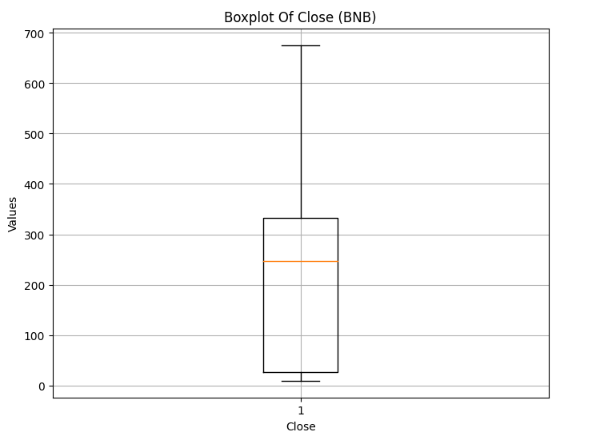
\includegraphics[width=1\textwidth]{Figure/BNBBoxplot.png}
    \caption{Biểu đồ Boxplot giá trị Close của Binance Coin(BNB)}
    \label{fig:1}
    \end{minipage}
    \hfill
    \begin{minipage}{0.23\textwidth}
    \centering
    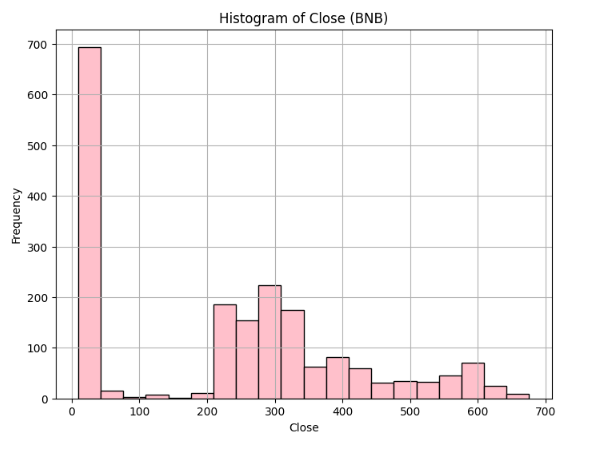
\includegraphics[width=1\textwidth]{Figure/BNBHistogram.png}
    \caption{Biểu đồ Histogram giá trị Close của Binance Coin(BNB)}
    \label{fig:2}
    \end{minipage}
\end{figure}
\begin{figure}[H]
    \centering
    \begin{minipage}{0.23\textwidth}
    \centering
    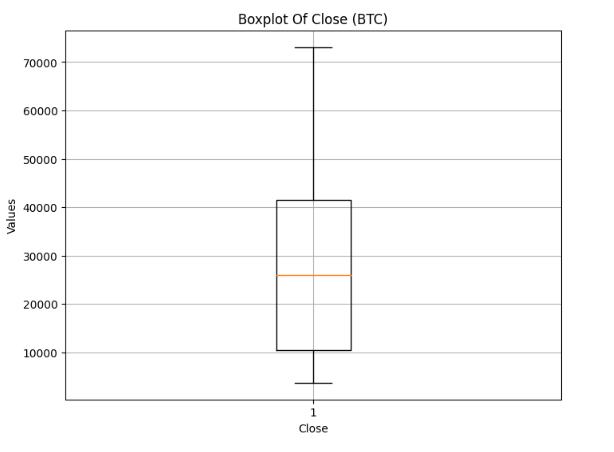
\includegraphics[width=1\textwidth]{Figure/BTCBoxplot.png}
    \caption{Biểu đồ Boxplot giá trị Close của Bitcoin (BTC)}
    \label{fig:1}
    \end{minipage}
    \hfill
    \begin{minipage}{0.23\textwidth}
    \centering
    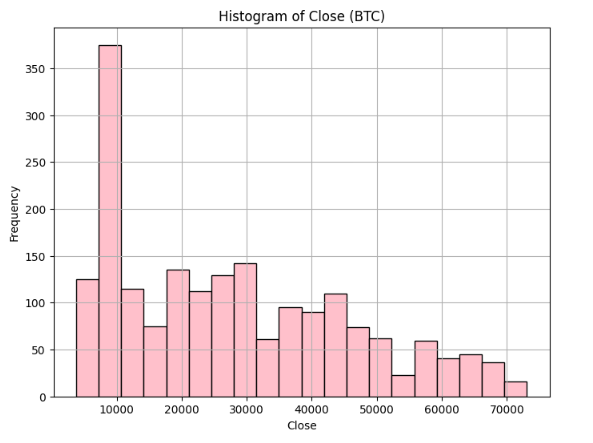
\includegraphics[width=1\textwidth]{Figure/BTCHistogram.png}
    \caption{Biểu đồ Histogram giá trị Close của Bitcoin (BTC)}
    \label{fig:2}
    \end{minipage}
\end{figure}

\begin{figure}[H]
    \centering
    \begin{minipage}{0.23\textwidth}
    \centering
    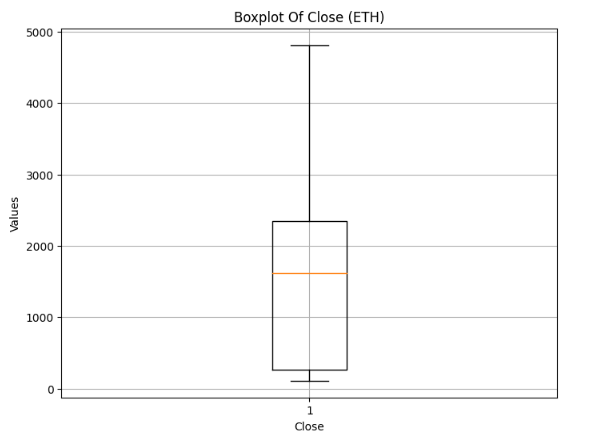
\includegraphics[width=1\textwidth]{Figure/ETHBoxplot.png}
    \caption{Biểu đồ Boxplot giá trị Close của Ethereum (ETH)}
    \label{fig:1}
    \end{minipage}
    \hfill
    \begin{minipage}{0.23\textwidth}
    \centering
    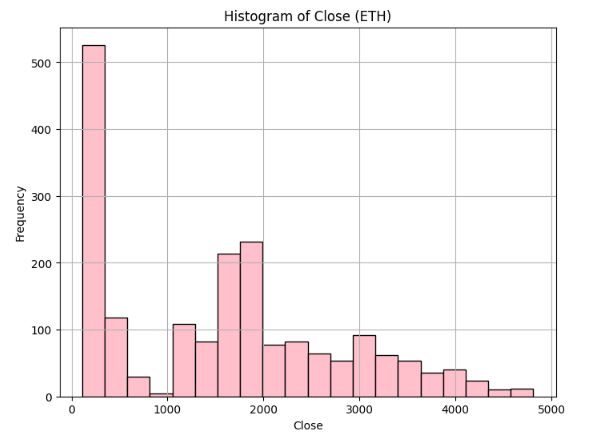
\includegraphics[width=1\textwidth]{Figure/ETHHistogram.png}
    \caption{Biểu đồ Histogram giá trị Close của Ethereum (ETH)}
    \label{fig:2}
    \end{minipage}
\end{figure}

\subsection{Công cụ}
Trong quá trình nghiên cứu, nhóm nhận thấy rằng có nhiều công cụ và thư viện Python phổ biến được sử dụng cho phân tích dữ liệu, hỗ trợ học sâu và trực quan hóa dữ liệu. Sau khi nghiên cứu và lựa chọn, nhóm quyết định sử dụng một số công cụ chính: numpy, pandas, sklearn, matplotlib.pyplot. Việc sử dụng những công cụ này đã giúp nhóm xác định dữ liệu, hiểu sâu hơn về ý nghĩa của dữ liệu. Đồng thời, khả năng trực quan hóa dữ liệu đã hỗ trợ đáng kể quá trình hiểu rõ chi tiết cũng như mô tả các bộ dữ liệu một cách rõ ràng, mang lại cái nhìn tổng quan rộng hơn trong việc khám phá dữ liệu.

\subsection{Tỉ lệ dữ liệu}
Trong quá trình phân tích dữ liệu chuỗi thời gian, nhóm chia tập dữ liệu thành các tập huấn luyện và kiểm tra bằng các tỷ lệ khác nhau: 70\% cho huấn luyện và 30\% cho kiểm tra, 80\% cho huấn luyện và 20\% cho kiểm tra, và 90\% cho huấn luyện và 10\% cho kiểm tra. Các tỷ lệ này giúp nhóm xem xét cách mà hiệu suất của mô hình bị ảnh hưởng bởi phân phối dữ liệu trong mỗi tập.\\

Tỷ lệ thông thường sử dụng là 7:3, dành 70\% cho huấn luyện và 30\% cho kiểm tra, tạo ra một sự cân bằng giữa việc cung cấp đủ dữ liệu huấn luyện và đảm bảo các tập dữ liệu khác biệt để điều chỉnh tinh chỉnh và đánh giá. Một lựa chọn khác là tỷ lệ 8:2, ưa chuộng tập huấn luyện 80\%, có lợi cho các mô hình phức tạp đòi hỏi một tập dữ liệu huấn luyện lớn hơn. Trong một số trường hợp, một cách tiếp cận cẩn thận như tỷ lệ 9:1 có thể được ưu tiên, đặc biệt là với một tập dữ liệu lớn và một mô hình đơn giản. Tỷ lệ này đảm bảo đủ dữ liệu huấn luyện trong khi cung cấp một tập kiểm tra đáng kể để đánh giá hiệu suất.

\subsection{Độ đo đánh giá mô hình}
RMSE: Sai số bình phương trung bình căn, đại diện cho căn bậc hai của sai số trung bình bình phương trong các giá trị yi dự đoán. Cơ bản, nó đo lường sự chênh lệch giữa các giá trị dự đoán và thực tế. Các giá trị RMSE thấp hơn cho thấy các mô hình dự đoán xuất sắc hơn.\\

MAPE: Là một phương pháp được sử dụng để đánh giá độ chính xác của một mô hình dự báo hoặc dự đoán. Nó tính toán sự lệch phần trăm trung bình giữa các giá trị dự đoán và thực tế, cung cấp một phép đo về hiệu suất của mô hình dựa trên sai số phần trăm.\\

MSE: Sai số bình phương trung bình, tính toán giá trị trung bình của sự khác biệt bình phương giữa các giá trị dự đoán và thực tế trong một mô hình. Nó cung cấp một phép đo về độ chính xác tổng thể bằng cách đo lường sự lớn mạnh của các sai số.\\

\[RMSE = \sqrt{\frac{\sum_{i=1}^{n} (y_i - \hat{y}_i)^2}{n}}\]\\

\[MAPE=\frac{100\%}{n}  \sum_{i=1}^{n} |\frac{y_i-\hat{y_i}}{y_i} | \]\\

\[MSE = \frac{\sum_{i=1}^{n} (y_i - \hat{y}_i)^2}{n}\]\\

Trong đó:\\
$$y_i \text{ is the observer value,}

$$\hat{y_i} \text{ is the predicted value,}

$$n \text{ is the number of observers}


\section{\textbf{Phương pháp luận}}
\subsection{RNN}
Mạng RNN (Recurrent Neural Network) là một dạng của mạng nơ-ron nhân tạo được thiết kế đặc biệt để xử lý dữ liệu chuỗi, trong đó mỗi dữ liệu đầu vào không chỉ phụ thuộc vào dữ liệu hiện tại mà còn phụ thuộc vào dữ liệu đã được xử lý trước đó trong chuỗi. Điều này giúp RNN hiểu và ánh xạ các mối quan hệ phức tạp giữa các thành phần trong chuỗi, như dữ liệu thời gian, ngôn ngữ tự nhiên, v.v.
\subsection{CCN-LSTM}
Mạng CNN-LSTM là một kiến trúc mạng nơ-ron sử dụng cả Convolutional Neural Network (CNN) và Long Short-Term Memory (LSTM). Mạng này kết hợp các lợi ích của cả hai loại mạng để xử lý dữ liệu chuỗi 2D hoặc 3D như hình ảnh hoặc video.\\
\textbf{Convolutional Neural Network (CNN):}\\
CNN thường được sử dụng để xử lý dữ liệu không gian như hình ảnh. Chúng sử dụng các lớp tích chập để trích xuất đặc trưng từ dữ liệu không gian bằng cách di chuyển các bộ lọc qua toàn bộ hình ảnh. Các lớp gộp được sử dụng để giảm kích thước của đặc trưng và tăng tính tổng quát của mô hình.\\
\textbf{Long Short-Term Memory (LSTM):}\\
LSTM thường được sử dụng để xử lý dữ liệu chuỗi thời gian như văn bản hoặc âm nhạc. Chúng có khả năng ghi nhớ thông tin từ quá khứ và lưu giữ nó trong trạng thái ẩn, cho phép mô hình hiểu các mối quan hệ phức tạp trong dữ liệu chuỗi.\\
\textbf{Kết hợp CNN và LSTM:}\\
Mạng CNN-LSTM kết hợp CNN để trích xuất đặc trưng không gian từ dữ liệu (ví dụ: các khối hình ảnh) và LSTM để hiểu mối quan hệ thời gian trong dữ liệu (ví dụ: chuỗi hình ảnh). Quá trình này cho phép mô hình hiểu được cả cấu trúc không gian và thời gian của dữ liệu, phù hợp cho nhiều ứng dụng như nhận dạng hình ảnh/video và dự báo chuỗi thời gian.\\
Mạng CNN-LSTM thường được sử dụng trong các lĩnh vực như xử lý hình ảnh/video, nhận dạng cử chỉ, dự báo thời tiết, dự báo chuỗi thời gian trong tài chính, và nhiều ứng dụng khác liên quan đến dữ liệu có cấu trúc không gian và thời gian.

\section{Thực nghiệm}

\subsection{Xây dựng mô hình}

\subsubsection{RNN}

\subsubsection{CNN-LSTM}
\begin{figure}[H]
    \centering
    \begin{minipage}{0.15\textwidth}
    \centering
    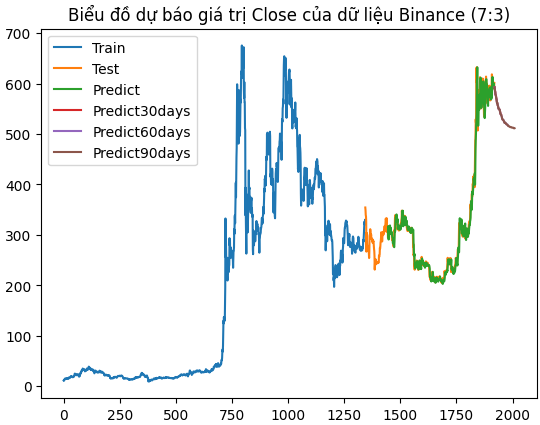
\includegraphics[width=1\textwidth]{Figure/RNN_BNB73.png}
    \end{minipage}
    \hfill
    \begin{minipage}{0.15\textwidth}
    \centering
    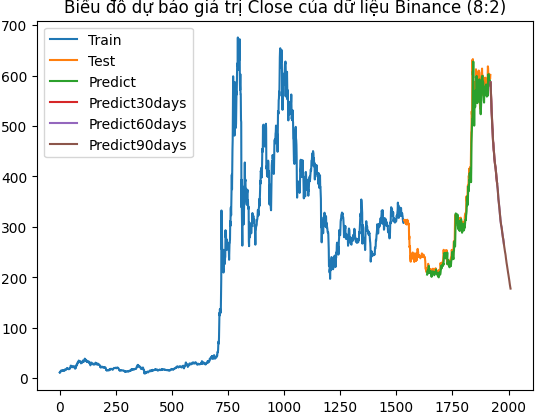
\includegraphics[width=1\textwidth]{Figure/RNN_BNB82.png}
    \end{minipage}
    \hfill
    \begin{minipage}{0.15\textwidth}
    \centering
    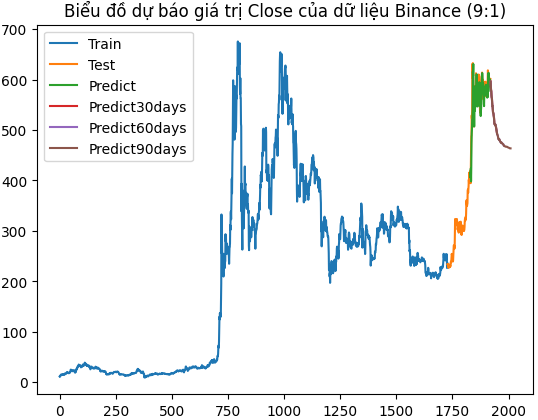
\includegraphics[width=1\textwidth]{Figure/RNN_BNB91.png}
    \end{minipage}
    \caption{Dữ liệu BNB-USD}
    \label{fig:1}
\end{figure}

\begin{figure}[H]
    \centering
    \begin{minipage}{0.15\textwidth}
    \centering
    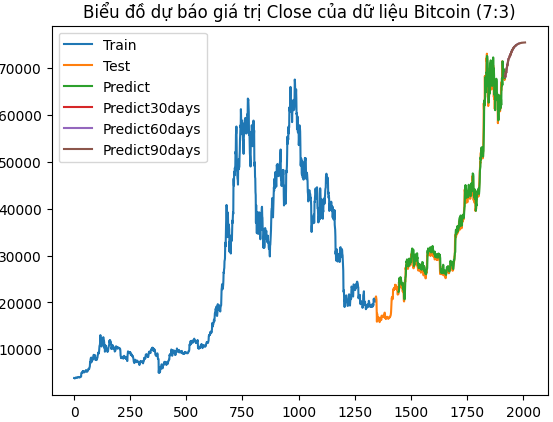
\includegraphics[width=1\textwidth]{Figure/RNN_BTC73.png}
    \end{minipage}
    \hfill
    \begin{minipage}{0.15\textwidth}
    \centering
    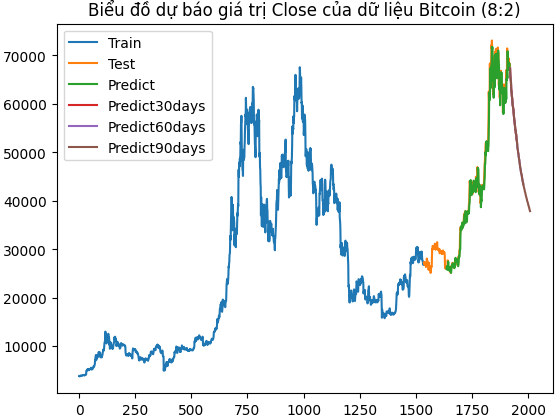
\includegraphics[width=1\textwidth]{Figure/RNN_BTC82.png}
    \end{minipage}
    \hfill
    \begin{minipage}{0.15\textwidth}
    \centering
    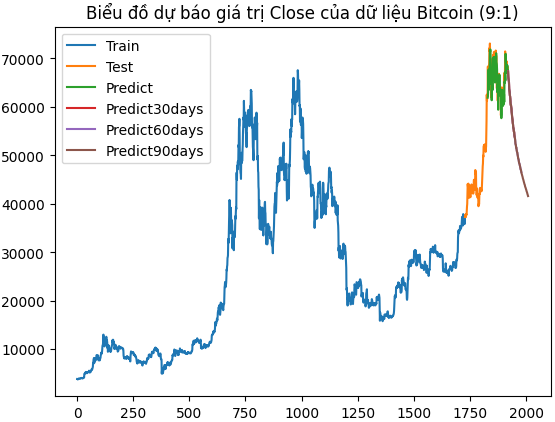
\includegraphics[width=1\textwidth]{Figure/RNN_BTC91.png}
    \end{minipage}
    \caption{Dữ liệu BTC-USD}
    \label{fig:1}
\end{figure}

\begin{figure}[H]
    \centering
    \begin{minipage}{0.15\textwidth}
    \centering
    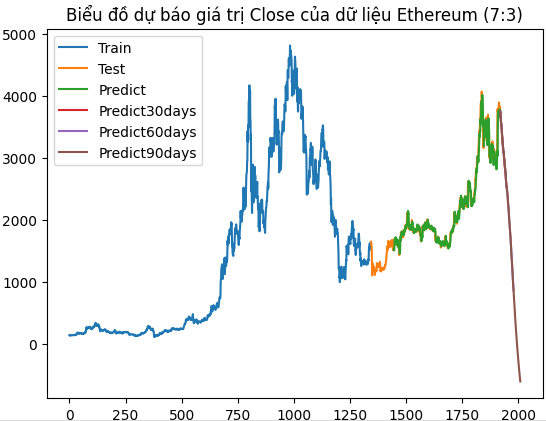
\includegraphics[width=1\textwidth]{Figure/RNN_ETH73.png}
    \end{minipage}
    \hfill
    \begin{minipage}{0.15\textwidth}
    \centering
    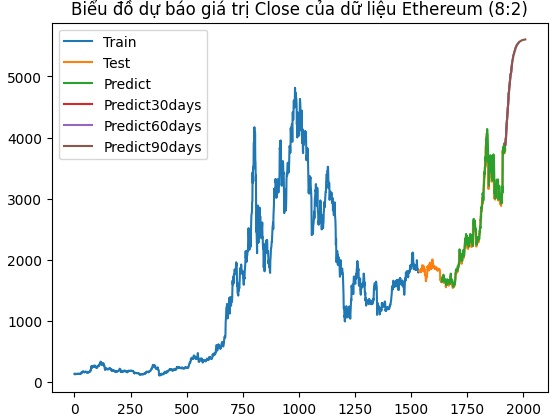
\includegraphics[width=1\textwidth]{Figure/RNN_ETH82.png}
    \end{minipage}
    \hfill
    \begin{minipage}{0.15\textwidth}
    \centering
    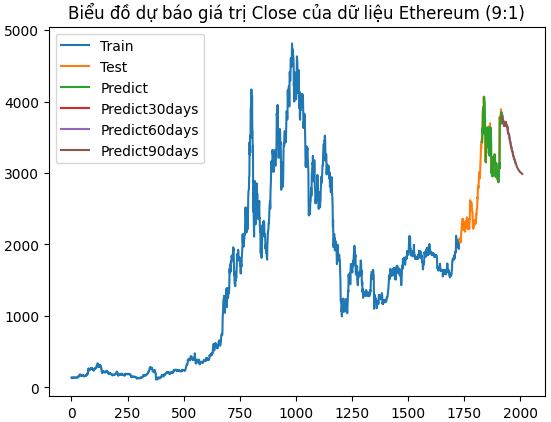
\includegraphics[width=1\textwidth]{Figure/RNN_ETH91.png}
    \end{minipage}
    \caption{Dữ liệu ETH-USD}
    \label{fig:1}
\end{figure}

\subsubsection{CNN-LSTM}

\begin{figure}[H]
    \centering
    \begin{minipage}{0.15\textwidth}
    \centering
    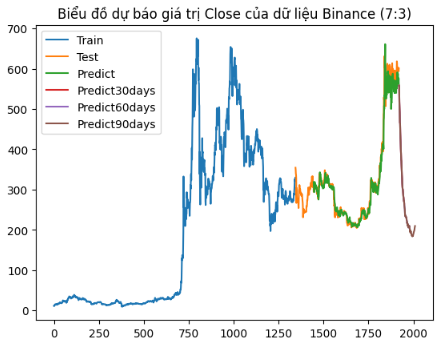
\includegraphics[width=1\textwidth]{Figure/BNB73.png}
    \end{minipage}
    \hfill
    \begin{minipage}{0.15\textwidth}
    \centering
    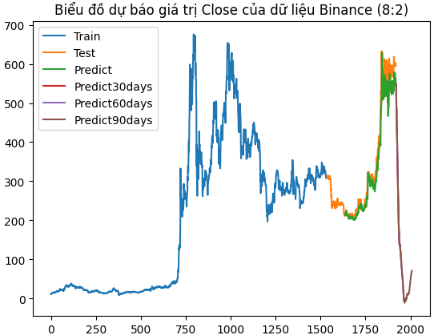
\includegraphics[width=1\textwidth]{Figure/BNB82.png}
    \end{minipage}
    \hfill
    \begin{minipage}{0.15\textwidth}
    \centering
    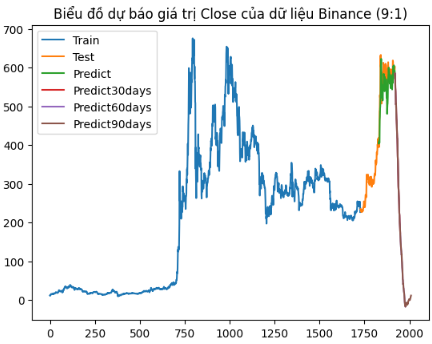
\includegraphics[width=1\textwidth]{Figure/BNB91.png}
    \end{minipage}
    \caption{Dữ liệu BNB-USD}
    \label{fig:1}
\end{figure}

\begin{figure}[H]
    \centering
    \begin{minipage}{0.15\textwidth}
    \centering
    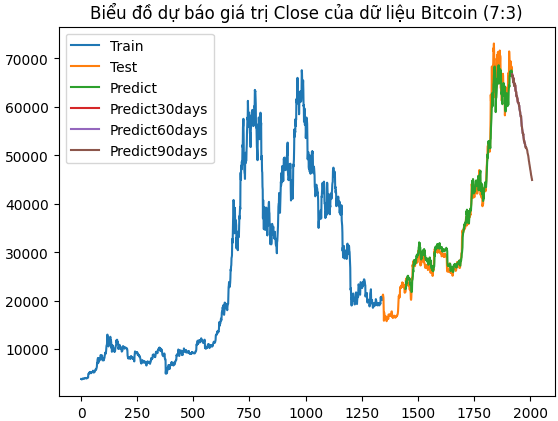
\includegraphics[width=1\textwidth]{Figure/BTC73.png}
    \end{minipage}
    \hfill
    \begin{minipage}{0.15\textwidth}
    \centering
    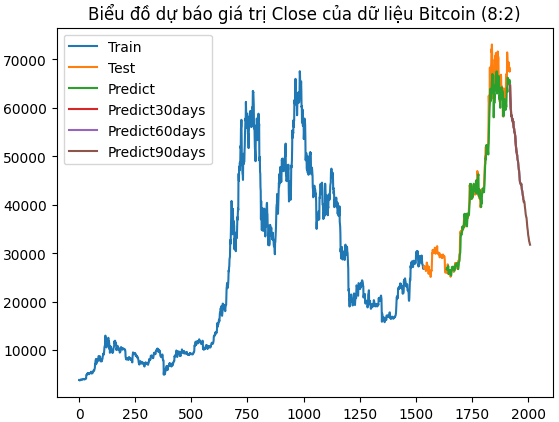
\includegraphics[width=1\textwidth]{Figure/BTC82.png}
    \end{minipage}
    \hfill
    \begin{minipage}{0.15\textwidth}
    \centering
    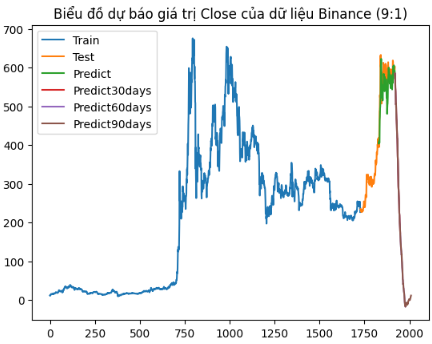
\includegraphics[width=1\textwidth]{Figure/BNB91.png}
    \end{minipage}
    \caption{Dữ liệu BTC-USD}
    \label{fig:1}
\end{figure}

\begin{figure}[H]
    \centering
    \begin{minipage}{0.15\textwidth}
    \centering
    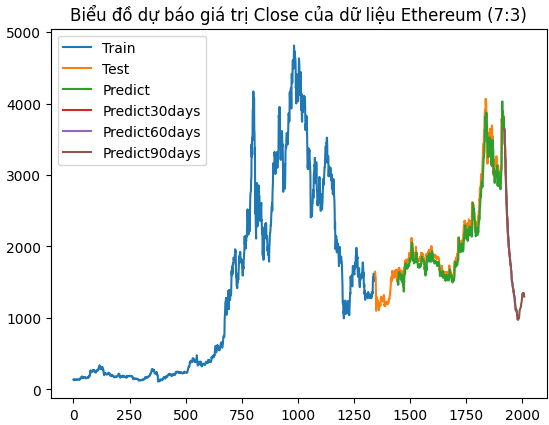
\includegraphics[width=1\textwidth]{Figure/ETH73.png}
    \end{minipage}
    \hfill
    \begin{minipage}{0.15\textwidth}
    \centering
    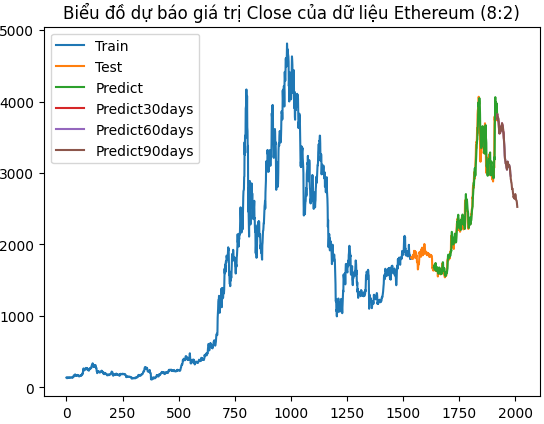
\includegraphics[width=1\textwidth]{Figure/ETH82.png}
    \end{minipage}
    \hfill
    \begin{minipage}{0.15\textwidth}
    \centering
    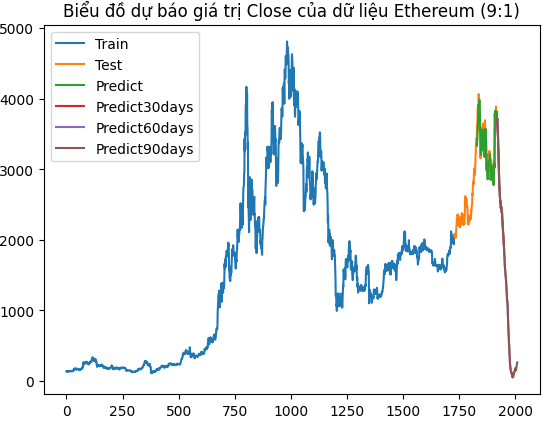
\includegraphics[width=1\textwidth]{Figure/ETH91.png}
    \end{minipage}
    \caption{Dữ liệu ETH-USD}
    \label{fig:1}
\end{figure}

\subsection{Độ đo đánh giá}

\begin{thebibliography}{9}

\bibitem{b1} Yecheng Yao, Jungho Yi, Shengjun Zhai, Yuwen Lin, Taekseung Kim Guihongxuan Zhang, Leonard Yoonjae Lee, “Predictive Analysis of Cryptocurrency Price Using Deep Learning”, International Journal of Engineering and Technology, Volume 7, Issue 3.27, pp. 258-264, 2018 [https://www.sciencepubco.com/index.php/ijet/article/view/17889]
\bibitem{b2} Muhammad Ali Nasir, Toan Luu Duc Huynh, Sang Phu Nguyen and Duy Duong, “Forecasting cryptocurrency returns and volume using search engines”, Financial Innovation 5, Article number 2, 2019 [https://jfin-swufe.springeropen.com/articles/10.1186/s40854-018-0119-8]
\bibitem{b3} Aggarwal A., Gupta I., Garg N., and Goel A., “Deep Learning Approach to Determine the Impact of Socio-Economic Factors on Bitcoin Price Prediction”, Twelfth International Conference on Contemporary Computing (IC3), 2019 [https://ieeexplore.ieee.org/document/8844928]
\bibitem{b4} Alessandretti, L.,ElBahrawy, A.,Aiello, L.M. and Baronchelli,A., 2018. Anticipating cryptocurrency prices using machine learning. Complexity, 2018. [https://www.hindawi.com/journals/complexity/2018/8983590/]
\bibitem{b5} Mittal R., Arora S. and Bhatia M. P. S., “Automated cryptocurrencies prices prediction using machine learning”, International Journal on Soft Computing, Volume 8, Issue 4, pp. 1758-1761, 2018
\bibitem{b6} Suhwan Ji, Jongmin KimORCID and Hyeonseung Im, “A Comparative Study of Bitcoin Price Prediction Using Deep Learning”, Department of Computer Science, Kangwon National University, Chuncheon-si, Gangwon-do 24341, Korea, 2019 [https://www.mdpi.com/2227-7390/7/10/898]
\bibitem{b7} Phumudzo Lloyd Seabe, Claude Rodrigue Bambe Moutsinga, andEdson Pindza, “Forecasting Cryptocurrency Prices Using LSTM, GRU, and Bi-Directional LSTM: A Deep Learning Approach”, 2023 [https://www.mdpi.com/2504-3110/7/2/203]
\bibitem{b8} Nguyen Dinh Thuan, Nguyen Minh Nhut, Hoang Tung, Vu Minh Sang, “PREDICTING THE CLOSING PRICE OF CRYPTOCURRENCY USING HYBRID ARIMA, REGRESSION AND MACHINE LEARNING”, Ky yeu Hoi nghi KHCN Quoc gia lan thu XIV ve Nghien cuu co ban va ung dung Cong nghe thong tin (FAIR), TP. HCM, ngay 23-24/12/2021

\end{thebibliography}

\end{document}
